
\begin{frame}
\frametitle{Laufzeitanalyse}
\framesubtitle{Fall 2}

\begin{enumerate}
	\item[1.] Den Improved-Graph $G'$ berechnen
	\item[1.1.] Alle I-simp.-Knoten von $G$ in Menge $SL$ zusammenfassen
\end{enumerate}
\ \\
\ \\

Wir definieren $Q = \{ ((v_i, v_j), - ) | (v_i, v_j) \in E, i < j \}$ \\
\hspace{2.86cm}$\cup \{ ((v_i, v_j), v) | v_i, v_j \in N_G(v), i < j \wedge deg(v) \leq k\}$ \\
\ \\
und $Q_{v_i,v_j} = \{ ((v_i, v_j), v) | v_i, v_j$ fest$, v \in V \} \subseteq Q$ \\



\end{frame}


\begin{frame}[t]
\frametitle{Laufzeitanalyse}
\framesubtitle{Fall 2}

\begin{columns}
	\column{.5\textwidth}
	\begin{block}{$Q$ für $k=2$:}
		\begin{itemize}
			\item $((1,3), -)$
			\item $((1,4), -)$
			\item $((1,5), -)$
			\item $((1,7), -)$
			\item $((2,4), -)$
			\item $((2,5), -)$
			\item $((2,6), -)$
			\item $((2,7), -)$
		\end{itemize}
	\end{block}
	
	\column{.5\textwidth}
	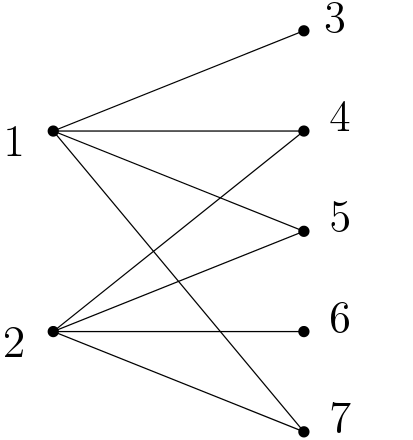
\includegraphics[width=0.7\textwidth]{images/Graph_Queue_1.png}
\end{columns}
\end{frame}

\begin{frame}[t]
\frametitle{Laufzeitanalyse}
\framesubtitle{Fall 2}

\begin{columns}
	\column{.5\textwidth}
	\begin{block}{$Q$:}
			\begin{itemize}
				\item $((1,3), -)$
				\item $((1,4), -)$
				\item $((1,5), -)$
				\item $((1,7), -)$
				\item $((2,4), -)$
				\item $((2,5), -)$
				\item $((2,6), -)$
				\item $((2,7), -)$
			
				\item $((1,2), 4)$
				\item $((1,2), 5)$
				\item $((1,2), 7)$
		\end{itemize}
	\end{block}

	\column{.5\textwidth}
		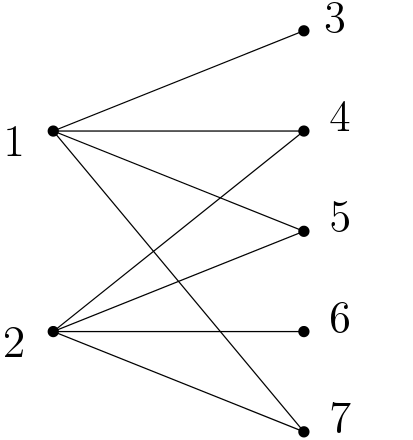
\includegraphics[width=0.7\textwidth]{images/Graph_Queue_1.png}
\end{columns}
\end{frame}

\begin{frame}[t]
\frametitle{Laufzeitanalyse}
\framesubtitle{Fall 2}

\begin{columns}
	\column{.5\textwidth}
	\begin{block}{$Q$, erster BucketSort:}
		\begin{itemize}
			\item $((1,3), -)$
			\item $((1,4), -)$
			\item $((1,5), -)$
			\item $((1,7), -)$
			\item $((1,2), 4)$
			\item $((1,2), 5)$
			\item $((1,2), 7)$
			\item $((2,4), -)$
			\item $((2,5), -)$
			\item $((2,6), -)$
			\item $((2,7), -)$
		\end{itemize}
	\end{block}
	
	\column{.5\textwidth}
	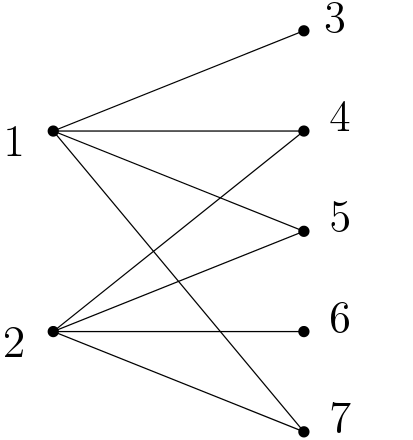
\includegraphics[width=0.7\textwidth]{images/Graph_Queue_1.png}
\end{columns}
\end{frame}


\begin{frame}[t]
\frametitle{Laufzeitanalyse}
\framesubtitle{Fall 2}

\begin{columns}
	\column{.5\textwidth}
	\begin{block}{$Q$, zweiter BucketSort:}
		\begin{itemize}
			\item $((1,2), 4)$
			\item $((1,2), 5)$
			\item $((1,2), 7)$
			\item $((1,3), -)$
			\item $((2,4), -)$
			\item $((1,4), -)$
			\item $((1,5), -)$
			\item $((2,5), -)$
			\item $((2,6), -)$
			\item $((1,7), -)$
			\item $((2,7), -)$
		\end{itemize}
	\end{block}
	
	\column{.5\textwidth}
	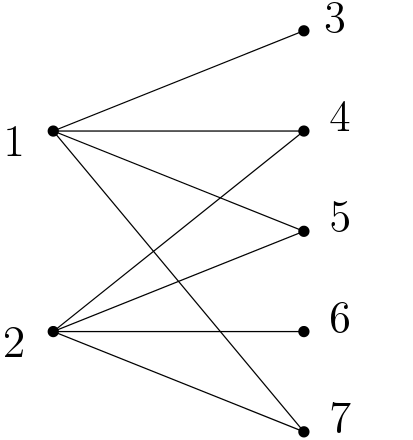
\includegraphics[width=0.7\textwidth]{images/Graph_Queue_1.png}
\end{columns}
\end{frame}


\begin{frame}
\frametitle{Laufzeitanalyse}
\framesubtitle{Fall 2}

$Q_{v_i,v_j} = \{ ((v_i, v_j), v) | v_i, v_j$ fest$, v \in V \} \subseteq Q$ \\
\ \\
Falls $|Q_{v_i, v_j}| \geq k \rightarrow (v_i, v_j) \in E'$, da $v_i$ und $v_j$ nun min. $(k+1)$ gemeinsame Nachbarn haben. \\
\ \\
Für jedes Element aus der oberen Menge und wenn $((v_i, v_j), -) \in Q$: \\
Füge $(v_i, v_j)$ für jedes $v \in V$ zu einer Menge $S_v$ hinzu, sodass $S_v$ alle Kanten von Nachbarn von $v$ enthält.\\
\end{frame}


\begin{frame}
\frametitle{Laufzeitanalyse}
\framesubtitle{Fall 2}

Der Graph $G' = (V,E')$ kann also aus den verschiedenen $Q_{v_i,v_j}$ ausgelesen werden. \\
\ \\
Das finden von I-simp.-Knoten ist durch $S_v$ nun auch möglich: Da alle Nachbarn von $v$ in $S_v$ sind, kann schnell geprüft werden ob $N_{G'}(v)$ eine Clique formt.

\end{frame}


\begin{frame}[t]
\frametitle{Laufzeitanalyse}
\framesubtitle{Fall 2}

\begin{columns}
	\column{.5\textwidth}
	\begin{block}{$Q$, zweiter BucketSort:}
		\begin{itemize}
			\item[1] $((1,2), 4)$
			\item[2] $((1,2), 5)$
			\item[3] $((1,2), 7)$
			\item $((1,3), -)$
			\item $((2,4), -)$
		\end{itemize}
	\vdots
	\ \\
	\ \\
	$S$: \\
	\begin{tabular}{| c | c | c | c | c | c | c |}
		\hline
		$S_1$ & $S_2$ & $S_3$ & $S_4$ & $S_5$ & $S_6$ & $S_7$ \\
		\hline
		{\scriptsize leer} & {\scriptsize leer} & {\scriptsize leer} & {\scriptsize leer} & {\scriptsize leer} & {\scriptsize leer} & {\scriptsize leer} \\
		\hline
	\end{tabular}
	\end{block}
	
	\column{.5\textwidth}
	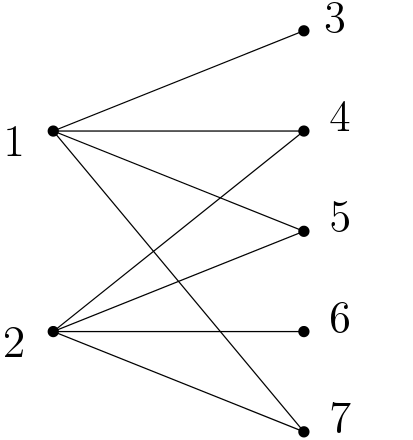
\includegraphics[width=0.7\textwidth]{images/Graph_Queue_1.png}
\end{columns}
\end{frame}


\begin{frame}
\frametitle{Laufzeitanalyse}
\framesubtitle{Fall 2}

Queue $Q$ für Menge $Q$, Array $S$ aus Listen für die $S_v$'s. \\
\ \\
\ \\

\begin{enumerate}
	\item Knoten ordnen $(v_1, v_2 \dots v_n)$
	\item $\forall (v_i, v_j) \in E, i < j:$ Lege $((v_i, v_j), -)$ auf $Q$
	\item $\forall v \in V:$ Lege alle $((v_i, v_j), v)$ mit $v_i, v_j \in N_G(v)$ und $i < j$ auf $Q$
	\item Bucket-sortiere $Q$ zwei mal: Ein mal nach dem ersten, dann nach zweiten Eintrag
\end{enumerate}


\end{frame}


\begin{frame}
\frametitle{Laufzeitanalyse}
\framesubtitle{Fall 2}

Sind nach dem Sortieren von $Q$ $(k+1)$ Einträge für gleiches $(v_i, v_j)$ in $Q$ untereinander $\rightarrow (v_i, v_j) \in E'$ \\
\ \\
Ist für solche $v_i, v_j$ auch $((v_i, v_j), -)$ in $Q$: Füge für jedes $((v_i, v_j), v)$ das Tupel $(v_i, v_j)$ in alle $S[v]$ ein.\\
\ \\
Ist in $S[v]$ jedes $v_i$ mit jedem $v_j$ verbunden: $N_G'(v)$ bildet Clique $\Rightarrow v$ ist I-simp. $\Rightarrow v \in SL$
\end{frame}


\begin{frame}[t]
\frametitle{Laufzeitanalyse}
\framesubtitle{Fall 2}


\begin{columns}
	\column{.5\textwidth}
	\begin{block}{$Q$, zweiter BucketSort:}
		\begin{itemize}
			\item[1] $((1,2), 4)$
			\item[2] $((1,2), 5)$
			\item[3] $((1,2), 7)$
			\item $((1,3), -)$
			\item $((2,4), -)$
		\end{itemize}
		\vdots
		\ \\
		\ \\
		$S$: \\
		\begin{tabular}{| c | c | c | c | c | c | c |}
			\hline
			$S_1$ & $S_2$ & $S_3$ & $S_4$ & $S_5$ & $S_6$ & $S_7$ \\
			\hline
			{\scriptsize leer} & {\scriptsize leer} & {\scriptsize leer} & {\scriptsize leer} & {\scriptsize leer} & {\scriptsize leer} & {\scriptsize leer} \\
			\hline
		\end{tabular}
	\end{block}
	
	\column{.5\textwidth}
	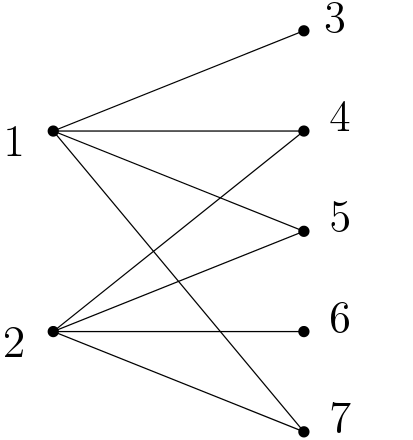
\includegraphics[width=0.7\textwidth]{images/Graph_Queue_1.png}
\end{columns}
\end{frame}


\begin{frame}
\frametitle{Laufzeitanalyse}
\framesubtitle{Fall 2}

\begin{enumerate}
	\item[2.] $SL$ von $G$ entfernen $\rightarrow \widehat{G}=(\widehat{V}, \widehat{E})$ entsteht %TODO Formulierung "Entsteht"?
	\item[3.] Algorithmus rekursiv auf $\widehat{G}$ ausführen
\end{enumerate}
\ \\
\ \\
\ \\
\ \\
Graph $\widehat{G}$ hat nach Entfernung von $SL$ $(1 - c_2) \cdot |V|$ Knoten. \\
\ \\
Wie in Fall 1 sind alle rekursiven Aufrufe in $O(|V|)$ möglich. \\

\end{frame}


\begin{frame}
\frametitle{Laufzeitanalyse}
\framesubtitle{Fall 2}

\begin{enumerate}
	\item[4.] Füge $SL$ wieder in die Zerteilung $(Y,T)$ ein
\end{enumerate}
\ \\
\ \\
\begin{enumerate}
	\item $\forall v \in SL$: Finde ein $Y_{i_v} \in Y$ in dem alle Nachbarn von $v$ sind ($N_G(v) \subseteq Y_{i_v}$)
	\item Füge $Y_{j_v} = \{ \{v\} \cup N_G(v) \}$ zu $Y$ hinzu und mache es adjazent zu $Y_{i_v}$ \\
	$\Rightarrow$ Baumzerteilung von $G$ mit Baumweite max. $k$
\end{enumerate}
\ \\



$Y_{i_v}$ existiert für jedes $v$, da I-simp.-Knoten in $G$ nicht adjazent sind und $N_G(v)$ eine Clique formt. \\
\ \\
\begin{KITinfoblock}{Lemma 2.1.i)}
	Ist $(X,T)$ Zerteilung von $G=(V,E)$ und $W \subseteq V$ formt Clique in $G \Rightarrow \exists i \in I: W \subseteq X_i$
\end{KITinfoblock}

\end{frame}


\begin{frame}
\frametitle{Laufzeitanalyse}
\framesubtitle{Fall 2}

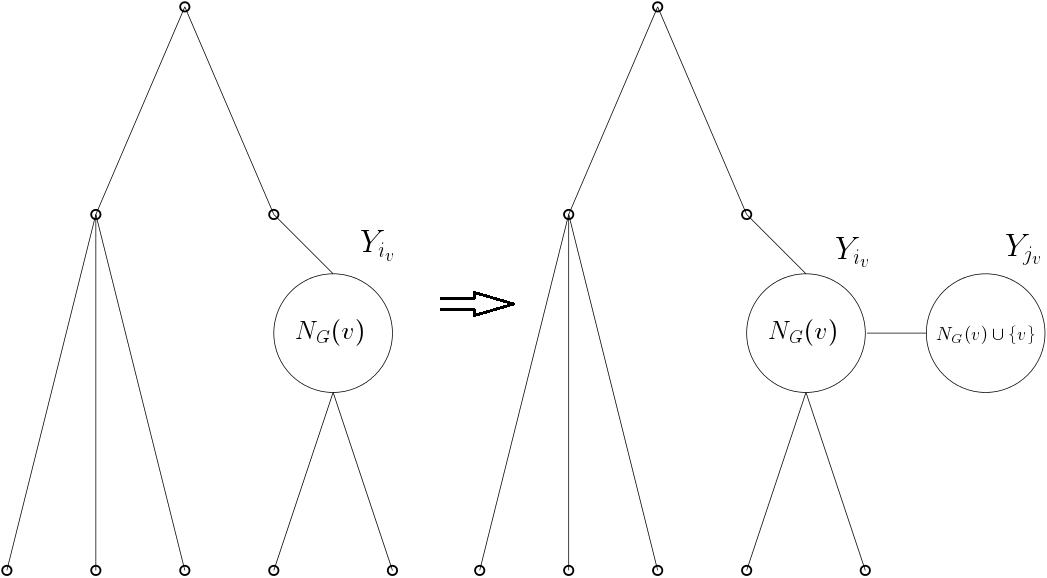
\includegraphics[width=0.95\textwidth]{images/Graph_zuruck.png}

\end{frame}



\begin{frame}
\frametitle{Laufzeitanalyse}
\framesubtitle{Fall 2}

\begin{itemize}
	\item Wir haben: $(Y,T)$ $k$-Zerteilung von $\widetilde{G}$
	\begin{itemize}
		\item $Y = \{ Y_i | i \in I \}$
	\end{itemize}

	\item Wir erstellen: $\forall l \in \{1 \dots k\}:$ Queue $Q_l$
	\begin{itemize}
		\item Also $k$ verschiedene Queues ($Q_1, Q_2 \dots Q_k$)
	\end{itemize}
\end{itemize}

\end{frame}


\begin{frame}
\frametitle{Laufzeitanalyse}
\framesubtitle{Fall 2}

\begin{enumerate}
	\item Queue $Q_l$: Füge alle Paare $((v_{i_1}, v_{i_2} \dots v_{i_l},), i)$ für alle $i \in I$ zu dieser Queue hinzu
	\begin{itemize}
		\item $v_{i_x} \in Y_i$
	\end{itemize}
	
	\item Füge zu $Q_l$ noch alle Paare $((v_{i_1}, v_{i_2} \dots v_{i_l},), v)$ mit $v \in SL$ und $v_{i_x} \in N_G(v)$ hinzu 
\end{enumerate}

\end{frame}

\begin{frame}
\frametitle{Laufzeitanalyse}
\framesubtitle{Fall 2}

\begin{columns}
	\column{0.25\textwidth}
	\begin{block}{}
		\textcolor{red}{$Q_1$}:
			\begin{itemize}
				\item[-] $((u_1), Y_1)$
				\item[-] $((v_1), Y_2)$
				\item[-] $((w_1), Y_3)$
				\item[-] $((x_1), Y_4)$
			\end{itemize}
		\textcolor{green}{$Q_2$}:
			\begin{itemize}
				\item[-] $((u_1, u_2), Y_1)$
				\item[-] $((v_1, v_2), Y_2)$
				\item[-] $((w_1, w_2), Y_3)$
				\item[-] $((x_1, x_2), Y_4)$
			\end{itemize}

	\end{block}

	\column{0.370\textwidth}
	\begin{block}{}
	\textcolor{cyan}{$Q_3$}:
		\begin{itemize}
			\item[-] $((u_1, u_2, u_3), Y_1)$
			\item[-] $((v_1, v_2, v_3), Y_2)$
			\item[-] $((w_1, w_2, w_3), Y_3)$
			\item[-] $((x_1, x_2, x_3), Y_4)$
		\end{itemize}
	\textcolor{purple}{$Q_4$}:
		\begin{itemize}
			\item[-] $((u_1, u_2, u_3, u_4), Y_1)$
			\item[-] $((v_1, u_2, v_3, v_4), Y_2)$
			\item[-] $((w_1, u_2, w_3, w_4), Y_3)$
			\item[-] $((x_1, u_2, x_3, x_4), Y_4)$
		\end{itemize}	
	\end{block}
	\column{.380\textwidth}
	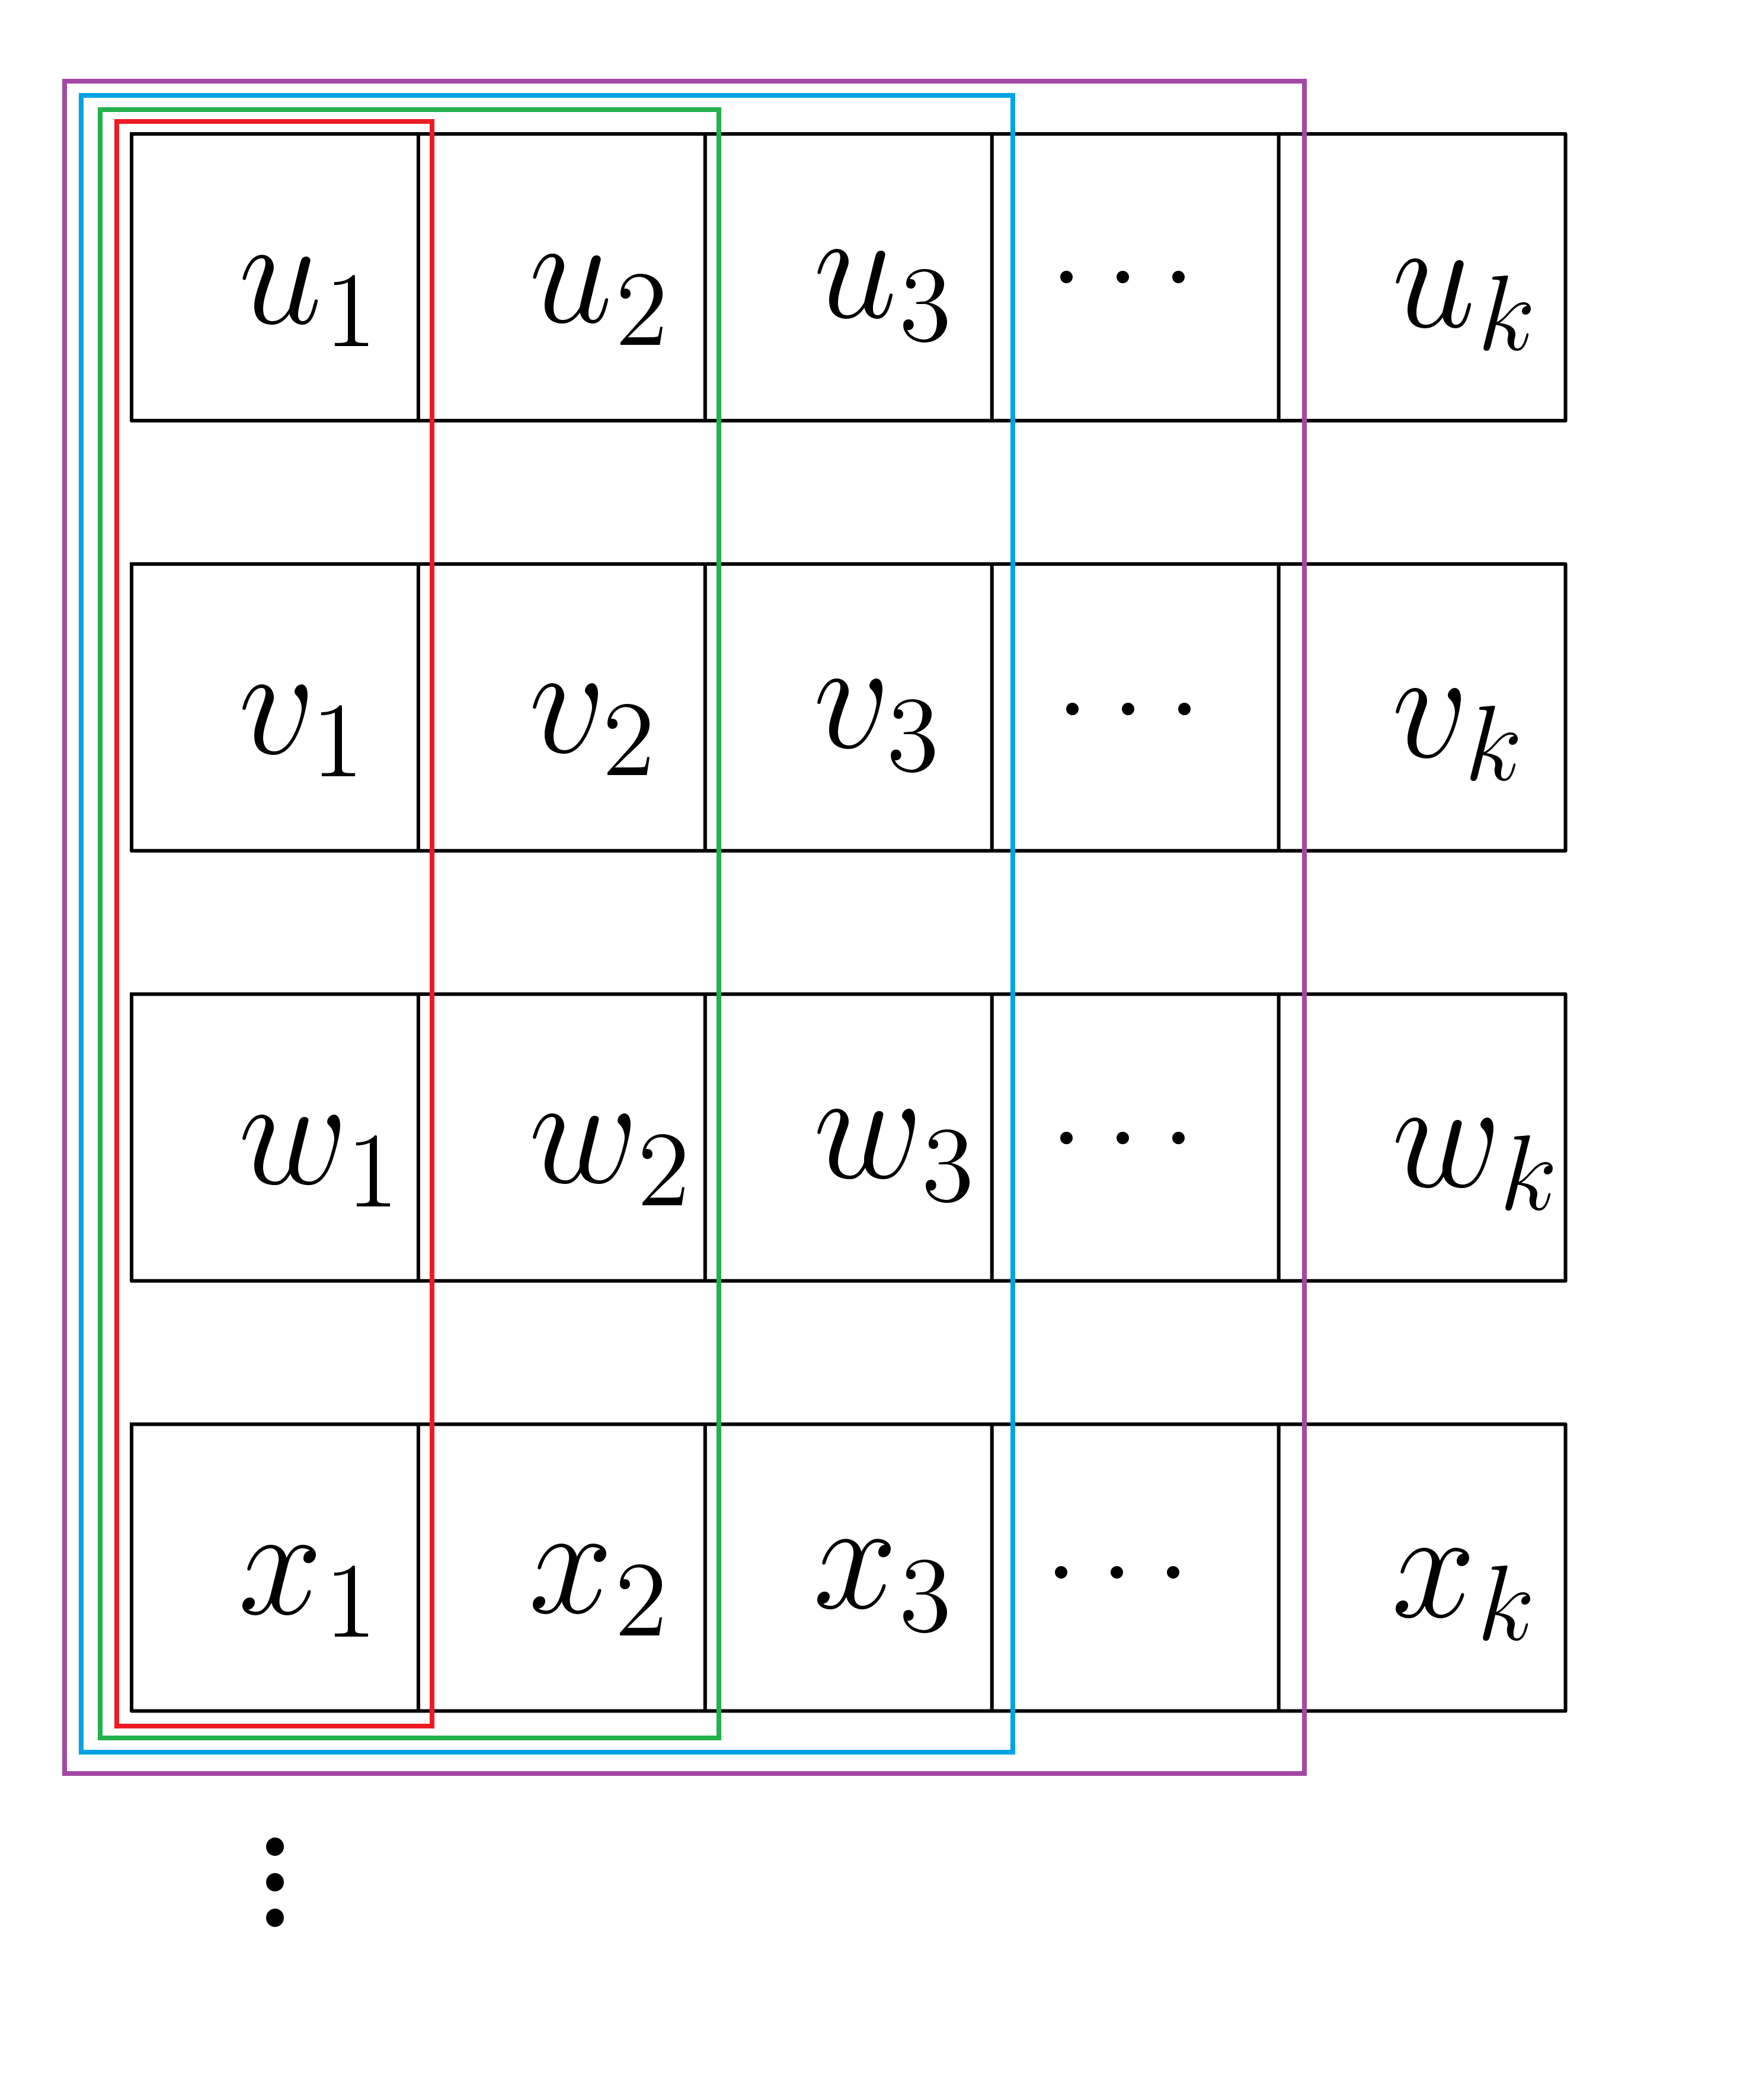
\includegraphics[width=1\textwidth]{images/Graph_Q-l_Farbe.png}

\end{columns}
\end{frame}

\begin{frame}
\frametitle{Laufzeitanalyse}
\framesubtitle{Fall 2}


Jedes $Q_l$ enthält nun die ersten $l$ Knoten jedes $Y_i \in Y$ und $l$ Nachbarn jedes $v \in SL$. \\
\ \\
\ \\
Bucket-sortiere jedes $Q_l$ $l$-mal, einmal für jeden Knoten $v_{i_x} \rightarrow$ Für jedes $((v_{i_1}, v_{i_2} \dots v_{i_l},), v)$ das passende Tupel $((v_{i_1}, v_{i_2} \dots v_{i_l},), i)$ adjazent in $Q$. \\
\ \\
So kann man den neuen Node direkt richtig erstellen und zu dem $Y_i$ adjazent machen. \\
\ \\

\end{frame}




















